\section{Machine-learning detectors}\label{sec:ml}

\subsection{Data set and models}
The labelled set is built from the same chunks and the same split: for each noise window of a split we also build a signal window, the \emph{same} window with a burst whose morphology is drawn uniformly among the three and whose optimal SNR is uniform in $[3,15]$. Classes are balanced and the label-0 windows contain all the real glitches and non-stationarity
($16\,224$ training and $8112$ validation windows per class, $8112$ test windows). A second training set contains only sine-Gaussians, to test generalisation to morphologies not seen in training. The networks see the whitened series clipped to $\pm12$ (glitches reach hundreds of $\sigma$); the feature pipeline uses the unclipped series.

\paragraph{Feature-based models.} Twenty-two morphology-agnostic features: the maximum over time of the z-scored sliding energy at five durations (the excess-power statistic at each scale), the maximum and the standard deviation over time of the energy in seven frequency sub-bands (30--500\,Hz, from a short-time spectrogram), and max\,$|v|$, kurtosis and std/MAD of the window. No matched-filter output is used.
\paragraph{CNN.} A one-dimensional convolutional network of $17\,761$ parameters: three Conv--BatchNorm--ReLU blocks (kernels 15, 9, 5; 16, 32, 64 channels; max-pooling by 4), global max-pooling (translation invariance: the burst can be anywhere), a dense layer with dropout $0.2$ and one logit; binary cross-entropy, Adam~\cite{Adam}, batch 128, early stopping on the validation loss (14 epochs). The \emph{ensemble} is five independently initialised copies (the logits are averaged); a second network is trained on sine-Gaussians only.
\paragraph{Autoencoder.} A convolutional autoencoder ($3.6\times10^5$ parameters, 32 latent values for 1024 samples) trained on the real noise windows \emph{only}; the reconstruction error is a morphology-independent anomaly score.

\subsection{Regularisation, bias--variance and what the features say}
Logistic regression with $L_1$ and $L_2$ penalties (Fig.~\ref{fig:reg}) reaches a validation AUC of $0.927$ with all features; the 5-fold cross-validated $L_1$ choice $C=0.019$ keeps 18 of the 22 features and costs nothing in AUC, while for $C\lesssim10^{-3}$ the $L_1$ model collapses much faster than $L_2$ (it sets coefficients to zero one by one).
Trees (Fig.~\ref{fig:bv}): the validation AUC of gradient boosting saturates at $0.938$ for depth 4--6 while the training AUC keeps rising ($0.936\to0.956$ from depth 1 to 12): beyond depth $\sim4$ there is only variance. The learning curve (depth 4) starts at a training AUC of $1.0$ against $0.925$ on validation with 500 examples, and the two approach each other ($0.952$ / $0.938$) at $3.2\times10^4$ examples without having converged: the feature models are data-limited, which is the practical argument for giving the network the raw series.
The most important features by permutation importance are the 10\,ms excess-power score and the energy in the 50--180\,Hz bands; the first principal component of the features carries 46\,\% of the variance. Validation AUCs: ridge $0.927$, random forest $0.938$, gradient boosting $0.938$.

\begin{figure}[h]\centering
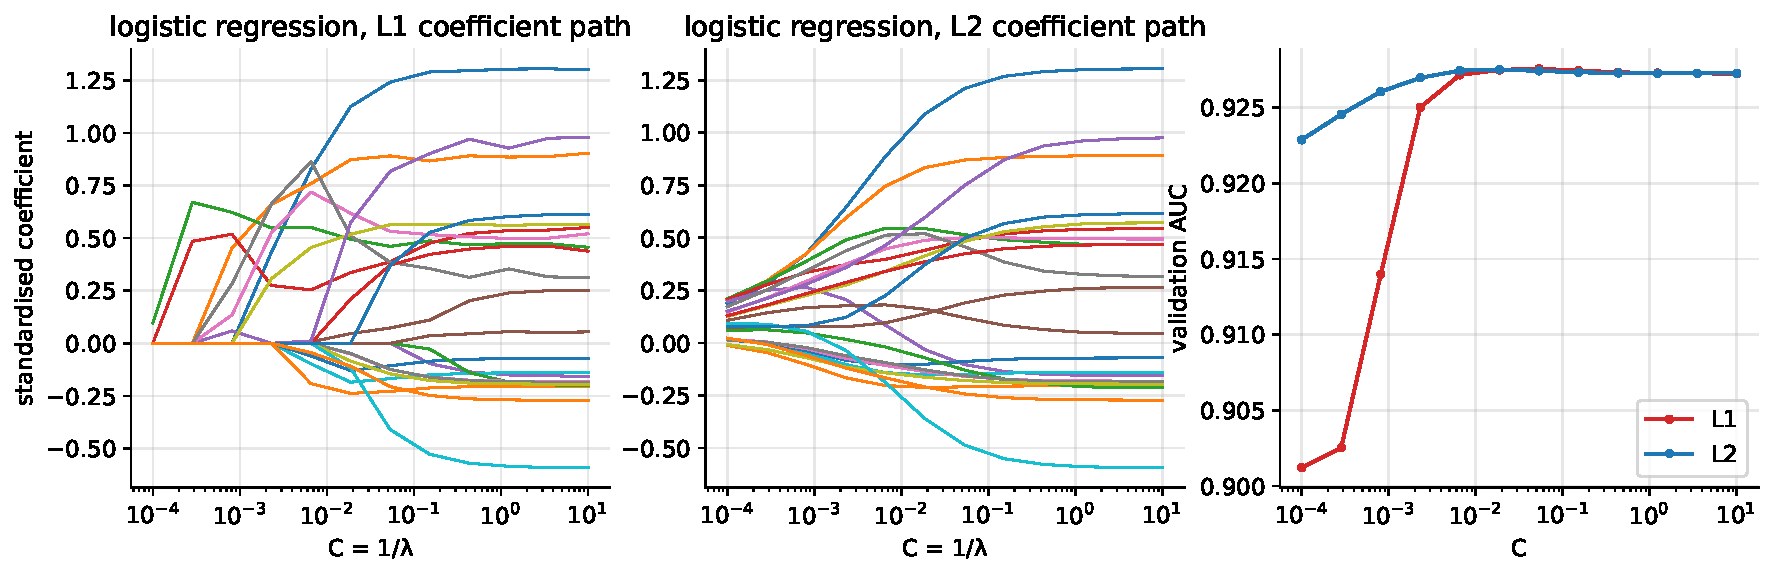
\includegraphics[width=0.95\textwidth]{fig05_regularization.pdf}\\[0.3em]
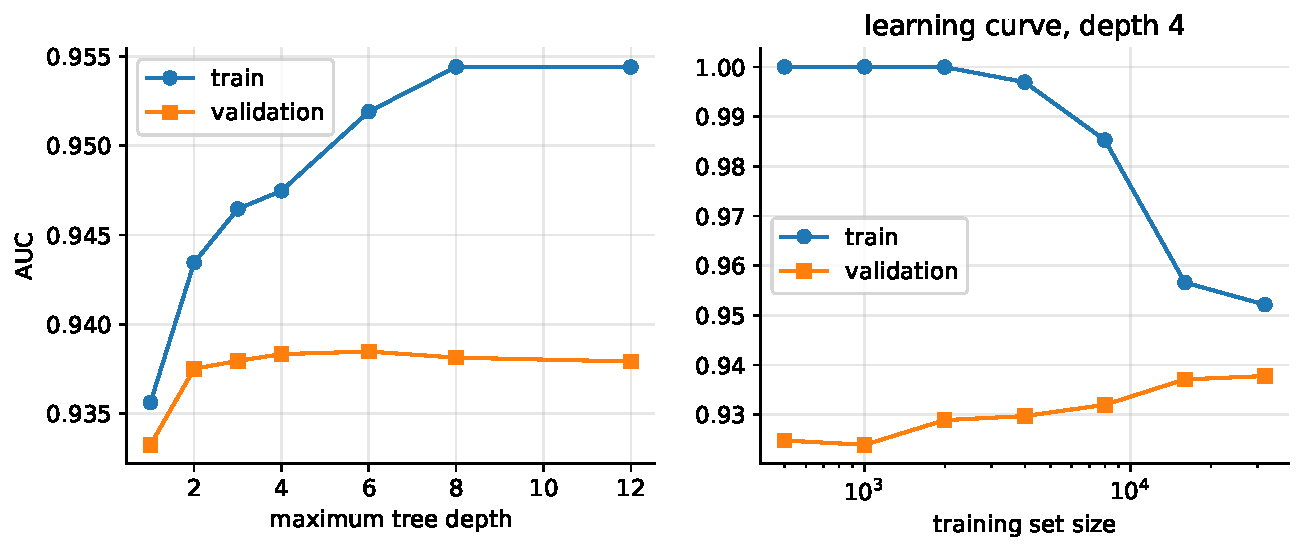
\includegraphics[width=0.62\textwidth]{fig05_bias_variance.pdf}
\caption{Top: $L_1$ and $L_2$ coefficient paths and validation AUC against $C$. Bottom: bias--variance (AUC against tree depth) and learning curve of gradient boosting.}\label{fig:reg}\label{fig:bv}
\end{figure}

\subsection{Comparison with the frequentist statistics on the same injections}
All statistics are evaluated on exactly the same test windows and injections, with the threshold of each set to the 99\,\% quantile of its own distribution on the \emph{same} background, the validation noise (chunks 1 and 5). A common background is what makes the comparison fair: Section~\ref{sec:freq} used the training chunks, whose glitchy chunk~2 gives a more conservative bank threshold
(there $\snr_{50}=5.5$ for sine-Gaussians; here $4.9$). Table~\ref{tab:mlcomp} and Fig.~\ref{fig:mleff} summarise the result; if the threshold is instead set on the test noise itself (equal observed FAP) the networks gain $0.4$--$0.6$ in $\snr_{50}$ (the test epochs are cleaner than the validation ones) and the bank only $0.04$, so that the ensemble then also beats the bank in family ($4.6$ against $4.8$); the conclusions for pulse and chirp and for the unseen morphology are unchanged.

\begin{table}[h]\centering\small
\begin{tabular}{lrrrrrr}
\toprule
& \multicolumn{2}{c}{sine-Gaussian} & \multicolumn{2}{c}{Gaussian pulse} & \multicolumn{2}{c}{linear chirp}\\
statistic & $\snr_{50}$ & $\snr_{90}$ & $\snr_{50}$ & $\snr_{90}$ & $\snr_{50}$ & $\snr_{90}$\\
\midrule
matched-filter bank & \textbf{4.87} & \textbf{6.53} & 5.34 & 6.82 & 6.28 & 8.21\\
excess power & 6.54 & 9.10 & 5.77 & 7.54 & 10.10 & 12.21\\
ridge-logistic (22 features) & 6.40 & 8.26 & 5.72 & 7.46 & 6.81 & 8.96\\
gradient boosting (22 features) & 5.61 & 7.30 & 5.70 & 7.24 & 6.06 & 7.73\\
CNN (mixed training) & 5.56 & 7.80 & 4.62 & 6.52 & 5.71 & 7.64\\
CNN ensemble (5) & 5.05 & 7.05 & \textbf{4.21} & \textbf{5.90} & \textbf{5.28} & \textbf{6.92}\\
CNN (sine-Gaussian only) & 5.09 & 6.87 & 6.50 & 12.93 & 6.80 & 10.82\\
autoencoder, window MSE & 12.09 & 15.14 & 12.44 & 15.06 & 12.32 & 15.14\\
autoencoder, local max & 6.89 & 8.80 & 6.75 & 8.53 & 8.30 & 11.08\\
\bottomrule
\end{tabular}
\caption{Optimal SNR at 50\,\% and 90\,\% efficiency (FAP $10^{-2}$ on validation noise, test injections). Bold: best in each column.}\label{tab:mlcomp}
\end{table}

\begin{figure}[h]\centering
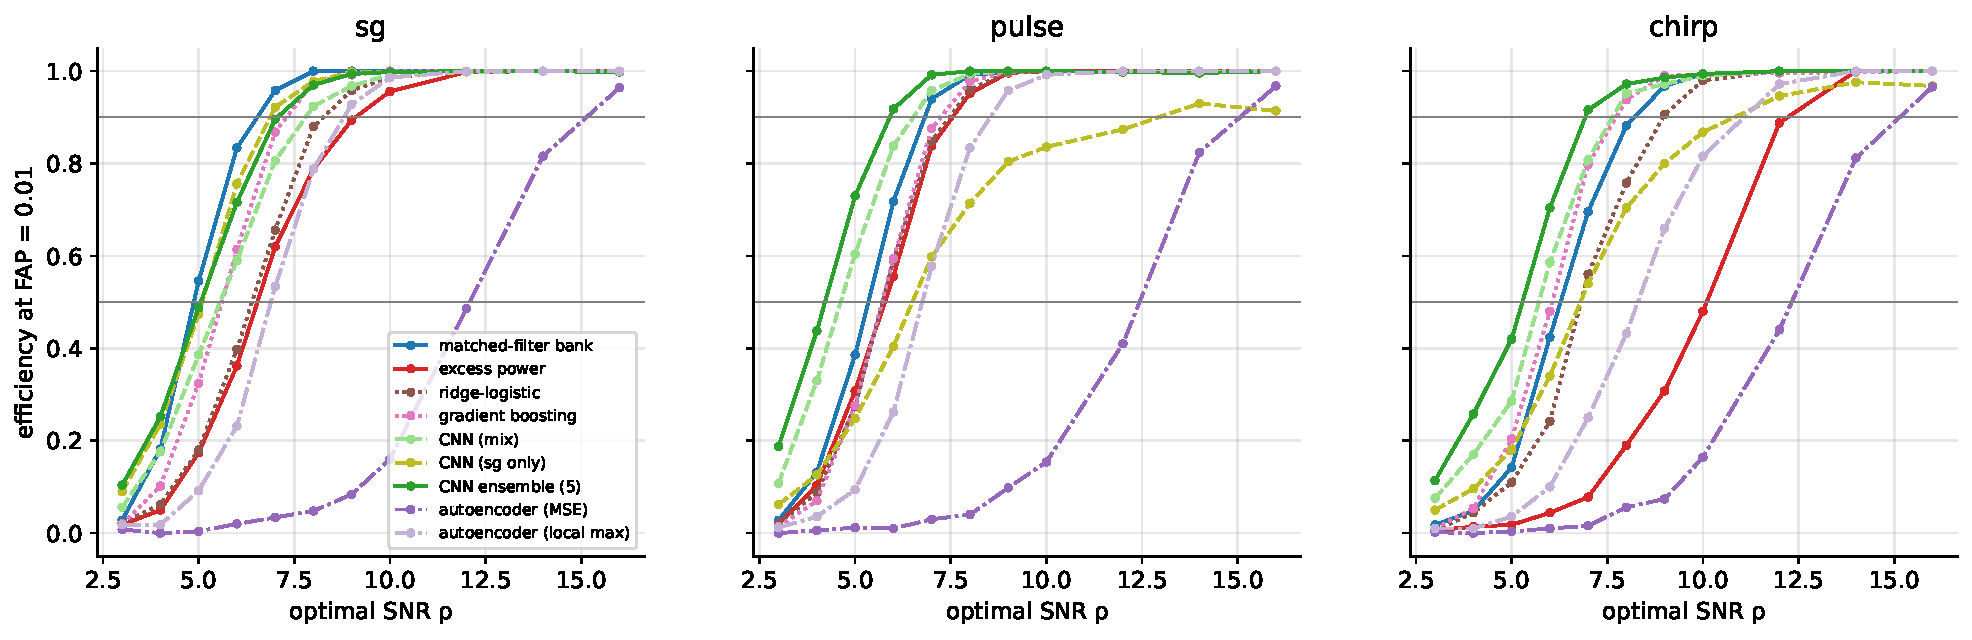
\includegraphics[width=\textwidth]{fig05_efficiency_all.pdf}
\caption{Efficiency against optimal SNR at FAP $10^{-2}$ for all statistics, on the same test injections.}\label{fig:mleff}
\end{figure}

\begin{itemize}[nosep]
\item \textbf{In family (sine-Gaussian).} The matched-filter bank and the ensemble are close ($\snr_{50}=4.9$ and $5.1$); the bank is better at 90\,\% ($6.5$ against $7.1$), the network wins by $0.2$ when the threshold is set on the test noise. Parity is a respectable result for a network that has seen no template.
\item \textbf{Morphologies in the training set (pulse, chirp).} The ensemble is about one unit of SNR better than the bank ($4.2$ against $5.3$; $5.3$ against $6.3$): it has \emph{learned} shapes that the bank covers only through its sine-Gaussian templates. Gradient boosting on 22 features is already at the bank level.
\item \textbf{A morphology not seen in training.} The CNN trained on sine-Gaussians only loses efficiency exactly where its training stops: $\snr_{50}=6.5$ (pulse) and $6.8$ (chirp) against $5.3$ and $6.3$ for the bank, and the efficiency at $\snr=8$ falls from $0.98$ to $0.71$ and $0.70$ (bank: $0.99$, $0.88$). The advantage of a supervised detector is bought with training data; outside the training distribution the bank, which has no data to fail on, is the more robust.
\item \textbf{Unsupervised.} The reconstruction error of the whole window is the total energy of a second of almost white noise --- there is nothing to learn --- and is inefficient ($\snr_{50}\approx12$). The \emph{local} maximum of the error recovers the performance of excess power ($6.9$, $6.8$, $8.3$) but not more: an autoencoder can beat an energy statistic only if the noise has structure that it can learn, which after whitening it hardly has.
\item \textbf{The CNN of this section is data-limited.} Section~\ref{sec:tuning} shows that training it with fresh injections at every epoch improves it by $\approx0.5$--$0.7$ in $\snr_{50}$ (a single network then beats the five-member ensemble); the numbers of this section are those of the static-data network, kept as the reference of the comparison.
\item \textbf{False alarms.} On the test chunks the observed FAP at a nominal $1\,\%$ is $0.85\,\%$ (bank), $0.92\,\%$ (excess power), $0.75\,\%$ (gradient boosting), $0.53\,\%$ (ensemble) and $0.35\,\%$ (single CNN): no statistic is immune to the epoch dependence of the background.
\end{itemize}

\subsection{Calibration and uncertainty}
A score is useful to a physicist if it is a probability. On balanced validation and test sets (noise plus mixed injections with SNR 3--15) all models are close to calibrated (Fig.~\ref{fig:cal}): the expected calibration error is $0.7\,\%$ for gradient boosting, $2.2$--$2.4\,\%$ for the CNNs and $2.7\,\%$ for the ridge model on the test set. The CNNs are slightly \emph{under}-confident at intermediate scores (observed signal fraction up to $\approx0.15$ above the prediction between $0.1$ and $0.7$).
Temperature scaling~\cite{Calibration} fitted on validation does not help ($T=0.94$--$1.02$; ECE changes by at most $0.002$): the miscalibration is not of the temperature type. For the CNNs the ECE is $0.8$--$1.2\,\%$ on the validation epochs they were tuned on and $2.2$--$2.4\,\%$ on the test epochs, so most of it is an \emph{epoch shift}. The ensemble is better than a single network in every proper score
(Brier $0.0350$ against $0.0413$, log-loss $0.110$ against $0.128$, AUC $0.9938$ against $0.9909$); the AUC on the test epochs is higher than on the validation ones for every model (ensemble $0.988\to0.994$), because the test chunks are cleaner: no sign of over-fitting to the training epochs.

The epistemic uncertainty is estimated with the ensemble~\cite{DeepEnsembles} and with MC dropout~\cite{MCDropout} ($30$ stochastic passes). The ensemble spread falls with SNR (mean std $0.16$ at $\snr\approx4$, $\approx0.001$ for $\snr\ge12$) and peaks at $p\approx0.5$; MC dropout shows the same trend but is only moderately correlated with it ($0.35$): they measure different things
(spread over dropout masks of one network against disagreement of independently trained networks). Rejecting the $20\,\%$ most uncertain windows raises the AUC from $0.9924$ to $0.9997$.

\begin{figure}[h]\centering
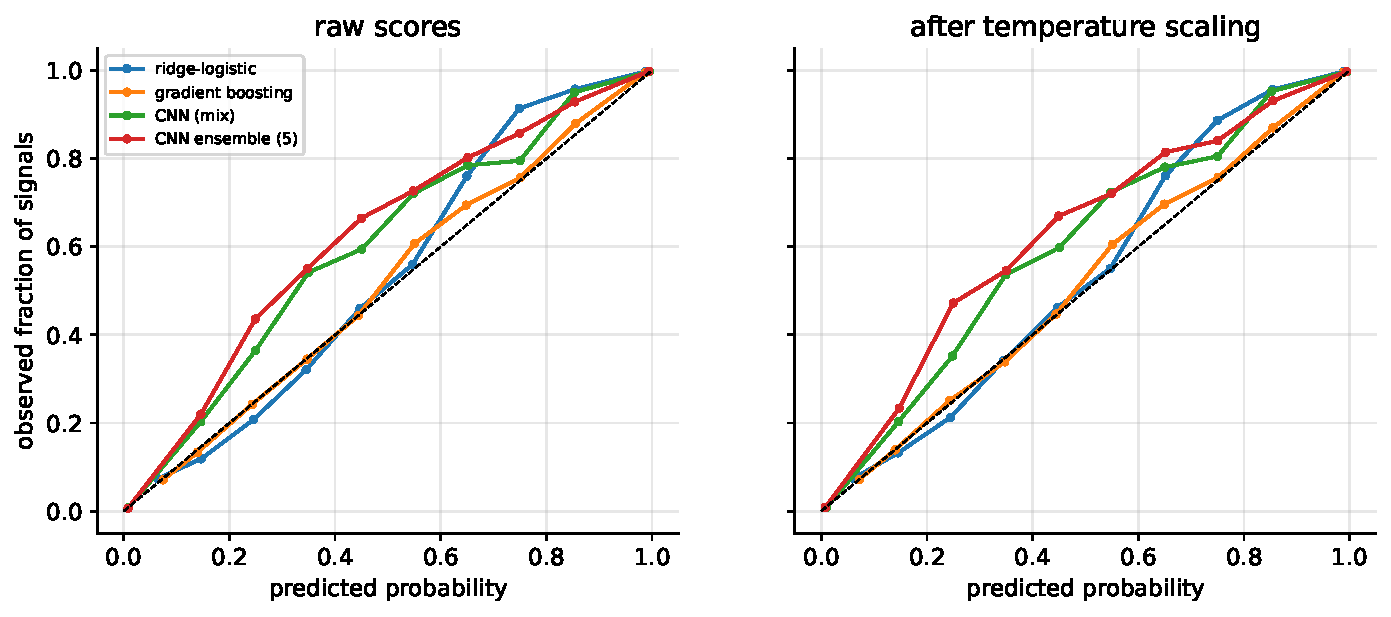
\includegraphics[width=0.78\textwidth]{fig05_calibration.pdf}\\[0.3em]
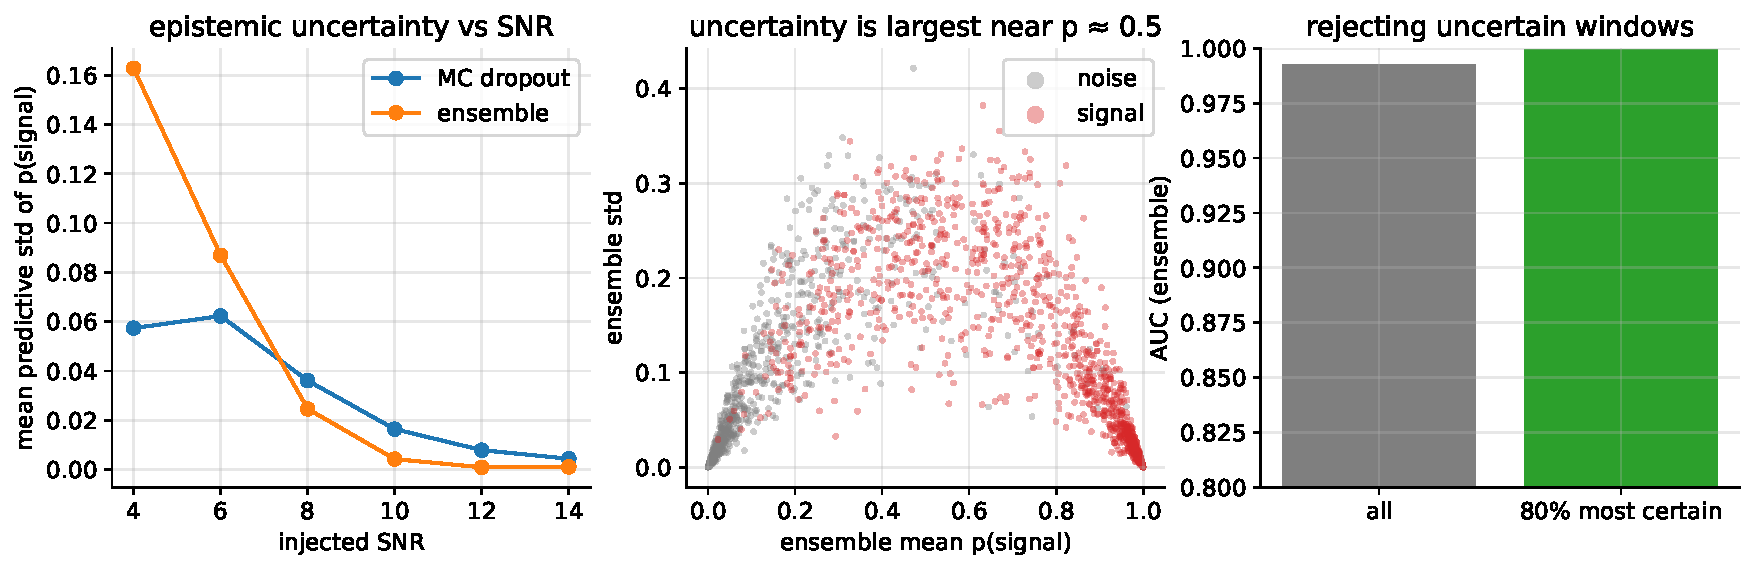
\includegraphics[width=0.95\textwidth]{fig05_uncertainty.pdf}
\caption{Top: reliability diagram on the test set, raw and after temperature scaling. Bottom: predictive standard deviation against SNR (ensemble and MC dropout), against the ensemble mean, and the effect of rejecting uncertain windows.}\label{fig:cal}
\end{figure}
